\documentclass[12pt]{article}
\usepackage{amsmath}
\usepackage{graphicx}
\usepackage{geometry}
\usepackage{fancyhdr}
\usepackage{float} % Package for strict H placement
\usepackage{rotating}

% --- Margin and Header Setup ---
\geometry{a4paper, margin=1in, top=1.2in} % Increased top margin slightly for the logo
\setlength{\headheight}{45pt} % Gives the header enough room for the image height

\pagestyle{fancy}
\fancyhf{} % Clears all default header and footer fields
\renewcommand{\headrulewidth}{0pt} % Removes the default horizontal line under the header

% Put the logo on the left and the page number on the right
\lhead{
\includegraphics[height=1.6cm]{images/guc_logo.png}} 
\rhead{\thepage}

\makeatletter
\setlength{\@fptop}{0pt}
\makeatother

\begin{document}

% ==========================================
%                 COVER PAGE
% ==========================================
\begin{titlepage}
    \thispagestyle{fancy} % Forces the header to show on the title page
    
    \vspace*{2cm}
    \begin{center}
        \textbf{\Huge Electric Circuits II Project} \\[1.5cm]
        \textbf{\Huge Report} \\[2.5cm]
        
        \large Prepared by \\[0.5cm]
        
        % The table for students
        \begin{tabular}{|c|c|}
            \hline
            \makebox[6cm]{Name} & \makebox[4cm]{ID} \\
            \hline
            Belal Nader Youssef & 64-11905 \\
            \hline
            Youssef Sameh Emil Shafik & 64-10650 \\
            \hline
        \end{tabular} \\[2.5cm]
        
        \large Tutorial Number \\[0.5cm]
        27
    \end{center}
\end{titlepage}

% ==========================================
%             REPORT CONTENT
% ==========================================
\setcounter{page}{2}
\newpage

\section*{Theoretical background:}
The chosen circuit is an \textbf{Inverting Active Band-Pass Filter}. It consists of an operational amplifier with a series resistor-capacitor network at the input ($R_1$ and $C_1$) and a parallel resistor-capacitor network in the feedback loop ($R_2$ and $C_2$).

\subsection*{Gain Equation Derivation (Phasor Domain)}
Assuming the non-inverting terminal ($V_p$) is connected to ground, making $V_p = 0$. Since the operational amplifier used is ideal, then $V_n = V_p = 0$.

Applying Nodal Analysis at node $V_n$:
\begin{equation}
    \frac{V_n - V_{in}}{Z_{in}} + \frac{V_n - V_{out}}{Z_f} = 0
\end{equation}

Expanding the impedances $Z_{in}$ (series $R_1, C_1$) and $Z_f$ (parallel $R_2, C_2$):
\begin{equation}
    \frac{V_n - V_{in}}{R_1 + \frac{1}{j\omega C_1}} + \frac{V_n - V_{out}}{\left(\frac{1}{R_2} + j\omega C_2\right)^{-1}} = 0
\end{equation}

Simplifying the impedance fractions:
\begin{equation}
    \frac{V_n - V_{in}}{\frac{1 + j\omega R_1C_1}{j\omega C_1}} + \frac{V_n - V_{out}}{\frac{R_2}{1 + j\omega R_2C_2}} = 0
\end{equation}

Substituting $V_n = 0$:
\begin{equation}
    \frac{-V_{in}}{\frac{1 + j\omega R_1C_1}{j\omega C_1}} + \frac{-V_{out}}{\frac{R_2}{1 + j\omega R_2C_2}} = 0
\end{equation}

Rearranging to solve for the voltage gain $H(j\omega) = \frac{V_{out}}{V_{in}}$:
\begin{equation}
    \frac{V_{out}}{\frac{R_2}{1 + j\omega R_2C_2}} = \frac{-V_{in}}{\frac{1 + j\omega R_1C_1}{j\omega C_1}} \implies \frac{V_{out}}{V_{in}} = - \frac{\frac{R_2}{1 + j\omega R_2C_2}}{\frac{1 + j\omega R_1C_1}{j\omega C_1}}
\end{equation}

\begin{equation}
    H(j\omega) = \frac{-j\omega R_2C_1}{(1 + j\omega R_1C_1)(1 + j\omega R_2C_2)}
\end{equation}

Expanding the denominator and separating real and imaginary parts:
\begin{equation}
    H(j\omega) = \frac{-j\omega R_2C_1}{(1 - \omega^2 R_1C_1 R_2C_2) + j\omega(R_1C_1 + R_2C_2)}
\end{equation}

\subsection*{Gain Magnitude and Resonant Frequency ($f_0$)}
The magnitude of the voltage gain $|H_v(j\omega)|$ is obtained by dividing the magnitude of the numerator by the magnitude of the denominator:
\begin{equation}
    |H(j\omega)| = \frac{\omega R_2C_1}{\sqrt{(1 - \omega^2 R_1C_1 R_2C_2)^2 + \omega^2(R_1C_1 + R_2C_2)^2}}
\end{equation}

To find the resonant frequency ($\omega_0$) where the gain is maximum, we can minimize the square of the inverse of the magnitude function. Let $u(\omega) = \frac{1}{|H(j\omega)|^2}$:
\begin{equation}
    u(\omega) = \frac{1 - 2\omega^2 R_1C_1 R_2C_2 + \omega^4 (R_1C_1 R_2C_2)^2 + \omega^2(R_1C_1 + R_2C_2)^2}{\omega^2 R_2^2C_1^2}
\end{equation}

Simplifying the expression into separate terms:
\begin{equation}
    u(\omega) = \frac{1}{\omega^2 R_2^2C_1^2} + \frac{\omega^2 (R_1C_1 R_2C_2)^2}{R_2^2C_1^2} + \text{Constant Terms}
\end{equation}

Differentiating $u(\omega)$ with respect to $\omega$ and equating to zero to find the minimum:
\begin{equation}
    \frac{du}{d\omega} = - \frac{2}{\omega^3 R_2^2C_1^2} + \frac{2\omega (R_1C_1 R_2C_2)^2}{R_2^2C_1^2} = 0
\end{equation}
\begin{equation}
    \frac{1}{\omega^3} = \omega (R_1C_1 R_2C_2)^2 \implies \omega_0^4 = \frac{1}{(R_1C_1 R_2C_2)^2}
\end{equation}
\begin{equation}
    \omega_0 = \frac{1}{\sqrt{R_1C_1 R_2C_2}} \implies f_0 = \frac{1}{2\pi \sqrt{R_1C_1 R_2C_2}}
\end{equation}

\newpage

\section*{Filter design:}
Based on the theoretical equations, the following component values were selected to achieve a target maximum gain between 1 and 10, operating in the kilohertz range for the hardware implementation.

\subsection*{Component Values}
\begin{itemize}
    \item Input Resistance ($R_1$): $1 \text{ k}\Omega$
    \item Feedback Resistance ($R_2$): $5.6 \text{ k}\Omega$
    \item Input Capacitance ($C_1$): $68 \text{ nF}$
    \item Feedback Capacitance ($C_2$): $5.6 \text{ nF}$
\end{itemize}

\subsection*{Calculated Parameters}
Using the selected component values, the expected theoretical parameters for the simulation and hardware implementation are as follows:

\textbf{1. Lower Cut-off Frequency ($f_L$):}
\begin{equation}
    f_L = \frac{1}{2\pi (1000)(68 \times 10^{-9})} \approx 2.34 \text{ kHz}
\end{equation}

\textbf{2. Upper Cut-off Frequency ($f_H$):}
\begin{equation}
    f_H = \frac{1}{2\pi (5600)(5.6 \times 10^{-9})} \approx 5.08 \text{ kHz}
\end{equation}

\textbf{3. Center/Resonant Frequency ($f_0$):}
\begin{equation}
    f_0 = \frac{1}{2\pi \sqrt{R_1C_1 R_2C_2}} = \frac{1}{2\pi\sqrt{ (1000)(68 \times 10^{-9})(5600)(5.6 \times 10^{-9})}} \approx 3.45 \text{ kHz}
\end{equation}

\textbf{4. Maximum Expected Gain ($|{\max}|$):}
Substituting $\omega_0$ into the magnitude equation yields the maximum gain:

\[
\omega_0=\frac{1}{\sqrt{R_1C_1R_2C_2}} \implies \omega_0^2=\frac{1}{R_1C_1R_2C_2}
\]
\[
|H(j\omega_0)|=\frac{\omega_0 R_2C_1}
{\sqrt{\left(1-\omega_0^2R_1C_1R_2C_2\right)^2+\omega_0^2\left(R_1C_1+R_2C_2\right)^2}}
\]
Substituting $\omega_0^2$ inside the real part of the denominator:
\[
|H(j\omega_0)|=
\frac{\omega_0 R_2C_1}
{\sqrt{
\left(1-\omega_0^2\left(\frac{1}{\omega_0^2}\right)\right)^2
+
\omega_0^2(R_1C_1+R_2C_2)^2
}}
\]
\[
|H(j\omega_0)|=
\frac{\omega_0 R_2C_1}
{\sqrt{
(1-1)^2
+
\omega_0^2(R_1C_1+R_2C_2)^2
}}
\]
\[
|H(j\omega_0)|=
\frac{\omega_0 R_2C_1}
{\omega_0(R_1C_1+R_2C_2)}
\]
\begin{equation}
    |H_{\max}| = \frac{R_2C_1}{R_1C_1 + R_2C_2}
\end{equation}
\begin{equation}
    |H_{\max}| = \frac{(5600)(68 \times 10^{-9})}{(1000)(68 \times 10^{-9}) + (5600)(5.6 \times 10^{-9})} \approx 3.83
\end{equation}

\textbf{5. Expected Gain at Cut-off Frequencies ($|H_{\omega_L}|$ and $|H_{\omega_H}|$):}
The lower cut-off frequency is dictated by the input network: $\omega_L = \frac{1}{R_1C_1}$. Substituting $\omega_L$ into the gain magnitude equation:
\[
|H(j\omega_L)| = \frac{\left(\frac{1}{R_1C_1}\right) R_2C_1}{\sqrt{\left(1 - \left(\frac{1}{R_1C_1}\right)^2 R_1C_1 R_2C_2\right)^2 + \left(\frac{1}{R_1C_1}\right)^2(R_1C_1 + R_2C_2)^2}}
\]
\[
|H(j\omega_L)| = \frac{\frac{R_2}{R_1}}{\sqrt{\left(1 - \frac{R_2C_2}{R_1C_1}\right)^2 + \left(1 + \frac{R_2C_2}{R_1C_1}\right)^2}}
\]
Expanding the binomials inside the square root ($1 - 2x + x^2 + 1 + 2x + x^2 = 2 + 2x^2$):
\[
|H(j\omega_L)| = \frac{\frac{R_2}{R_1}}{\sqrt{2 + 2\left(\frac{R_2C_2}{R_1C_1}\right)^2}} = \frac{R_2C_1}{\sqrt{2((R_1C_1)^2 + (R_2C_2)^2)}}
\]
Similarly, substituting the upper cut-off frequency $\omega_H = \frac{1}{R_2C_2}$ yields an identical simplified expression due to the mathematical symmetry of the poles:
\[
|H(j\omega_H)| = \frac{\frac{C_1}{C_2}}{\sqrt{\left(1 - \frac{R_1C_1}{R_2C_2}\right)^2 + \left(\frac{R_1C_1}{R_2C_2} + 1\right)^2}} = \frac{R_2C_1}{\sqrt{2((R_1C_1)^2 + (R_2C_2)^2)}}
\]
Therefore, the exact theoretical gain at both cut-off frequencies is identical. Substituting the component values:
\begin{equation}
    |H_{\omega_L}| = |H_{\omega_H}| = \frac{(5600)(68 \times 10^{-9})}{\sqrt{2((1000 \cdot 68 \times 10^{-9})^2 + (5600 \cdot 5.6 \times 10^{-9})^2)}} \approx 3.60
\end{equation}

\newpage

\section*{Circuit simulation:}
The band-pass filter circuit was constructed using PSpice simulation software. The following figures detail the schematic diagram and the simulation profiles used for both AC sweep and transient (time-domain) analysis.

% --- Schematic Diagram ---
\begin{figure}[H]
    \centering
    \rotatebox{90}{
        \begin{minipage}{0.82\textheight} 
            \centering
            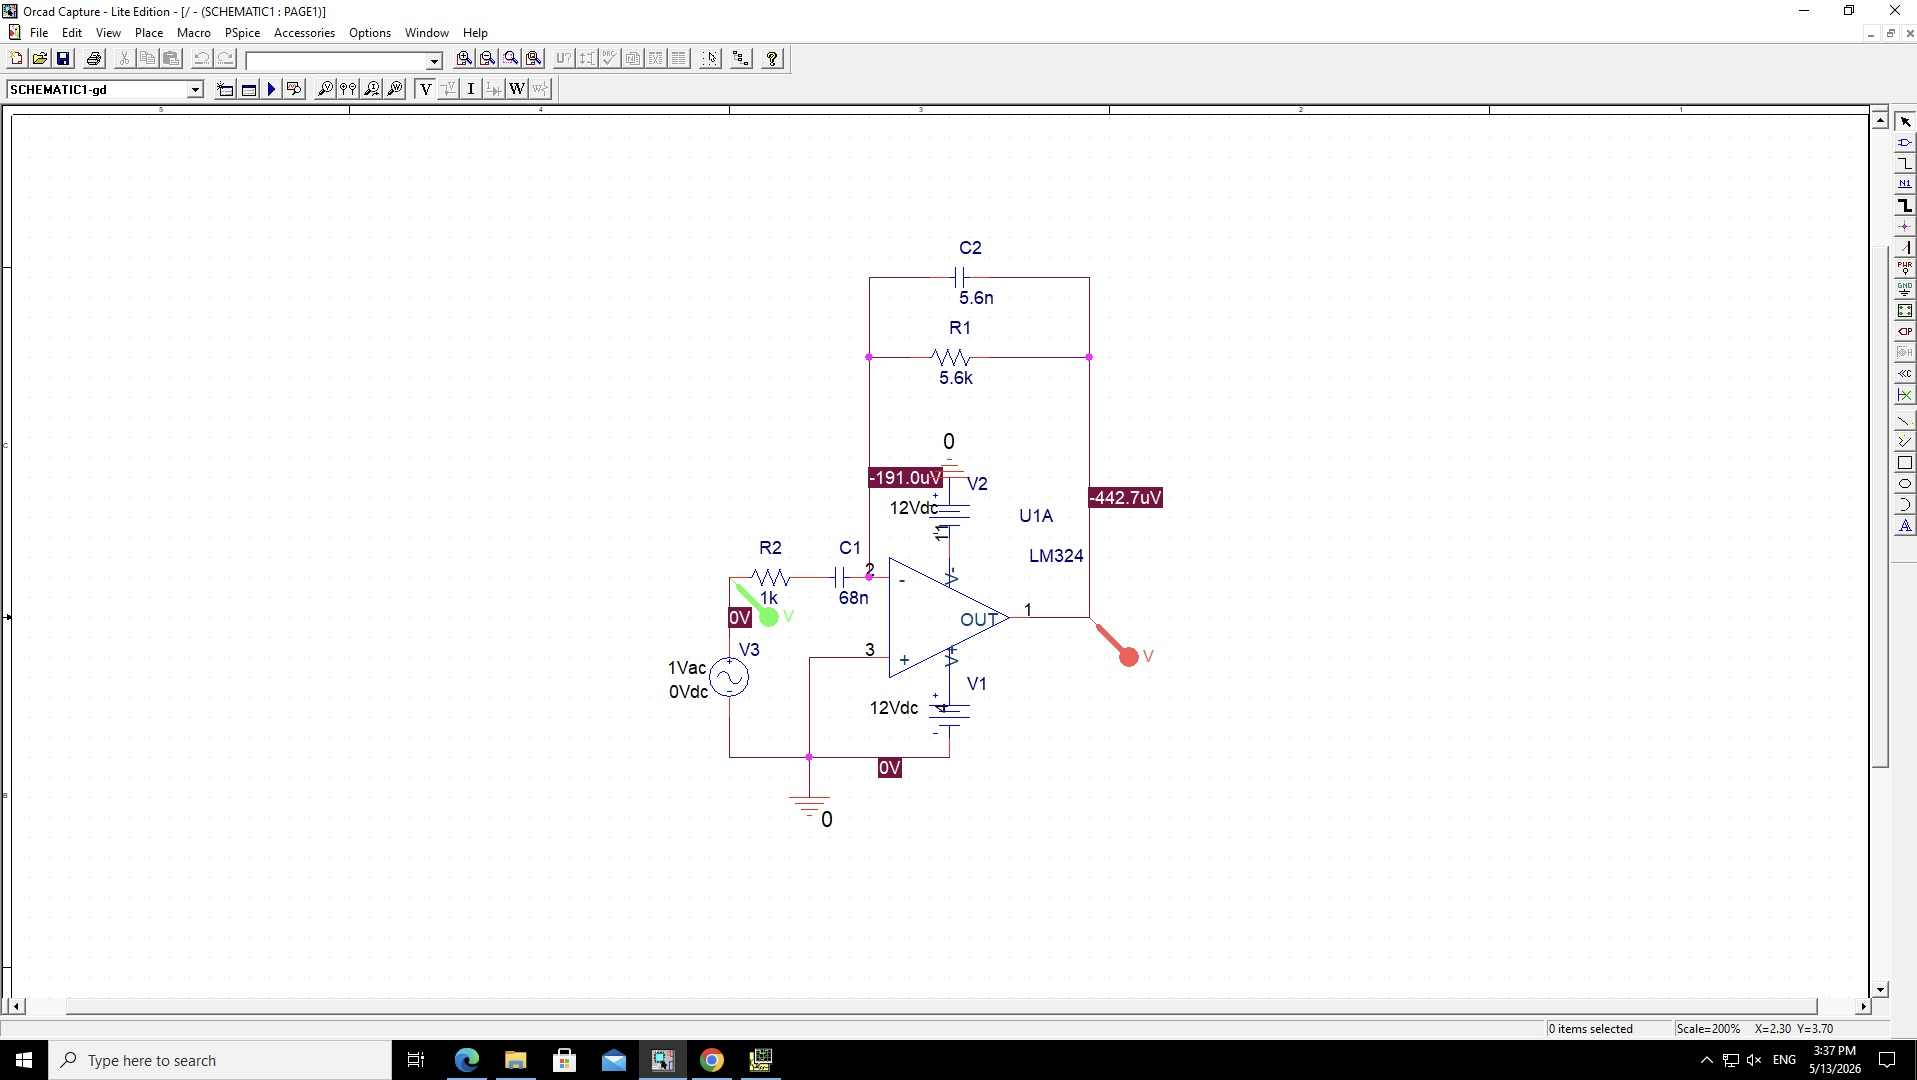
\includegraphics[width=\linewidth, keepaspectratio]{images/ac_shematic.png}
            \caption{PSpice schematic diagram of the Inverting Band-Pass Filter.}
            \label{fig:ac_schem}
        \end{minipage}
    }
\end{figure}

% --- Simulation Profile ---
\begin{figure}[H]
    \centering
    \rotatebox{90}{
        \begin{minipage}{1\textheight} 
            \centering
            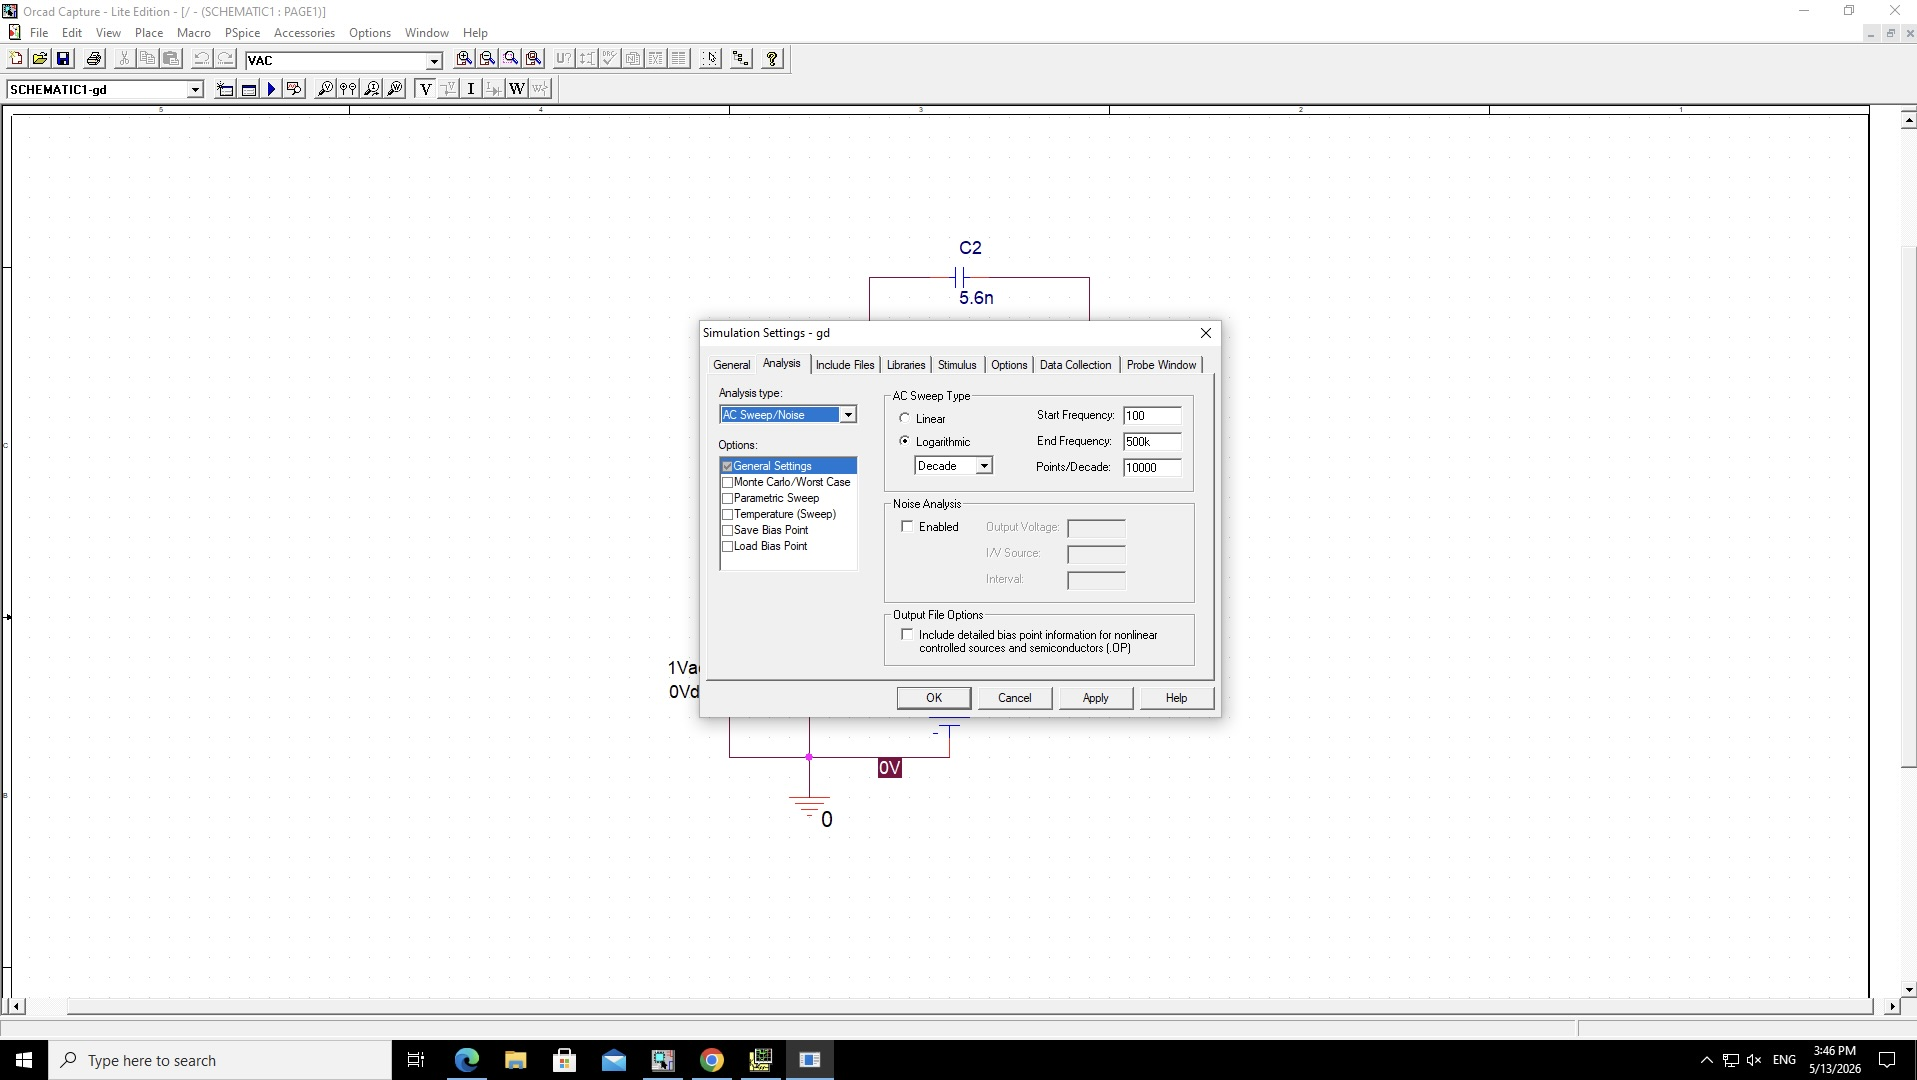
\includegraphics[width=\linewidth, keepaspectratio]{images/sweep_prof.png}
            \caption{AC Sweep simulation profile settings as mentioned in the project description.}
            \label{fig:hw_center}
        \end{minipage}
    }
\end{figure}

\begin{figure}[H]
    \centering
    \rotatebox{90}{
        \begin{minipage}{1\textheight} 
            \centering
            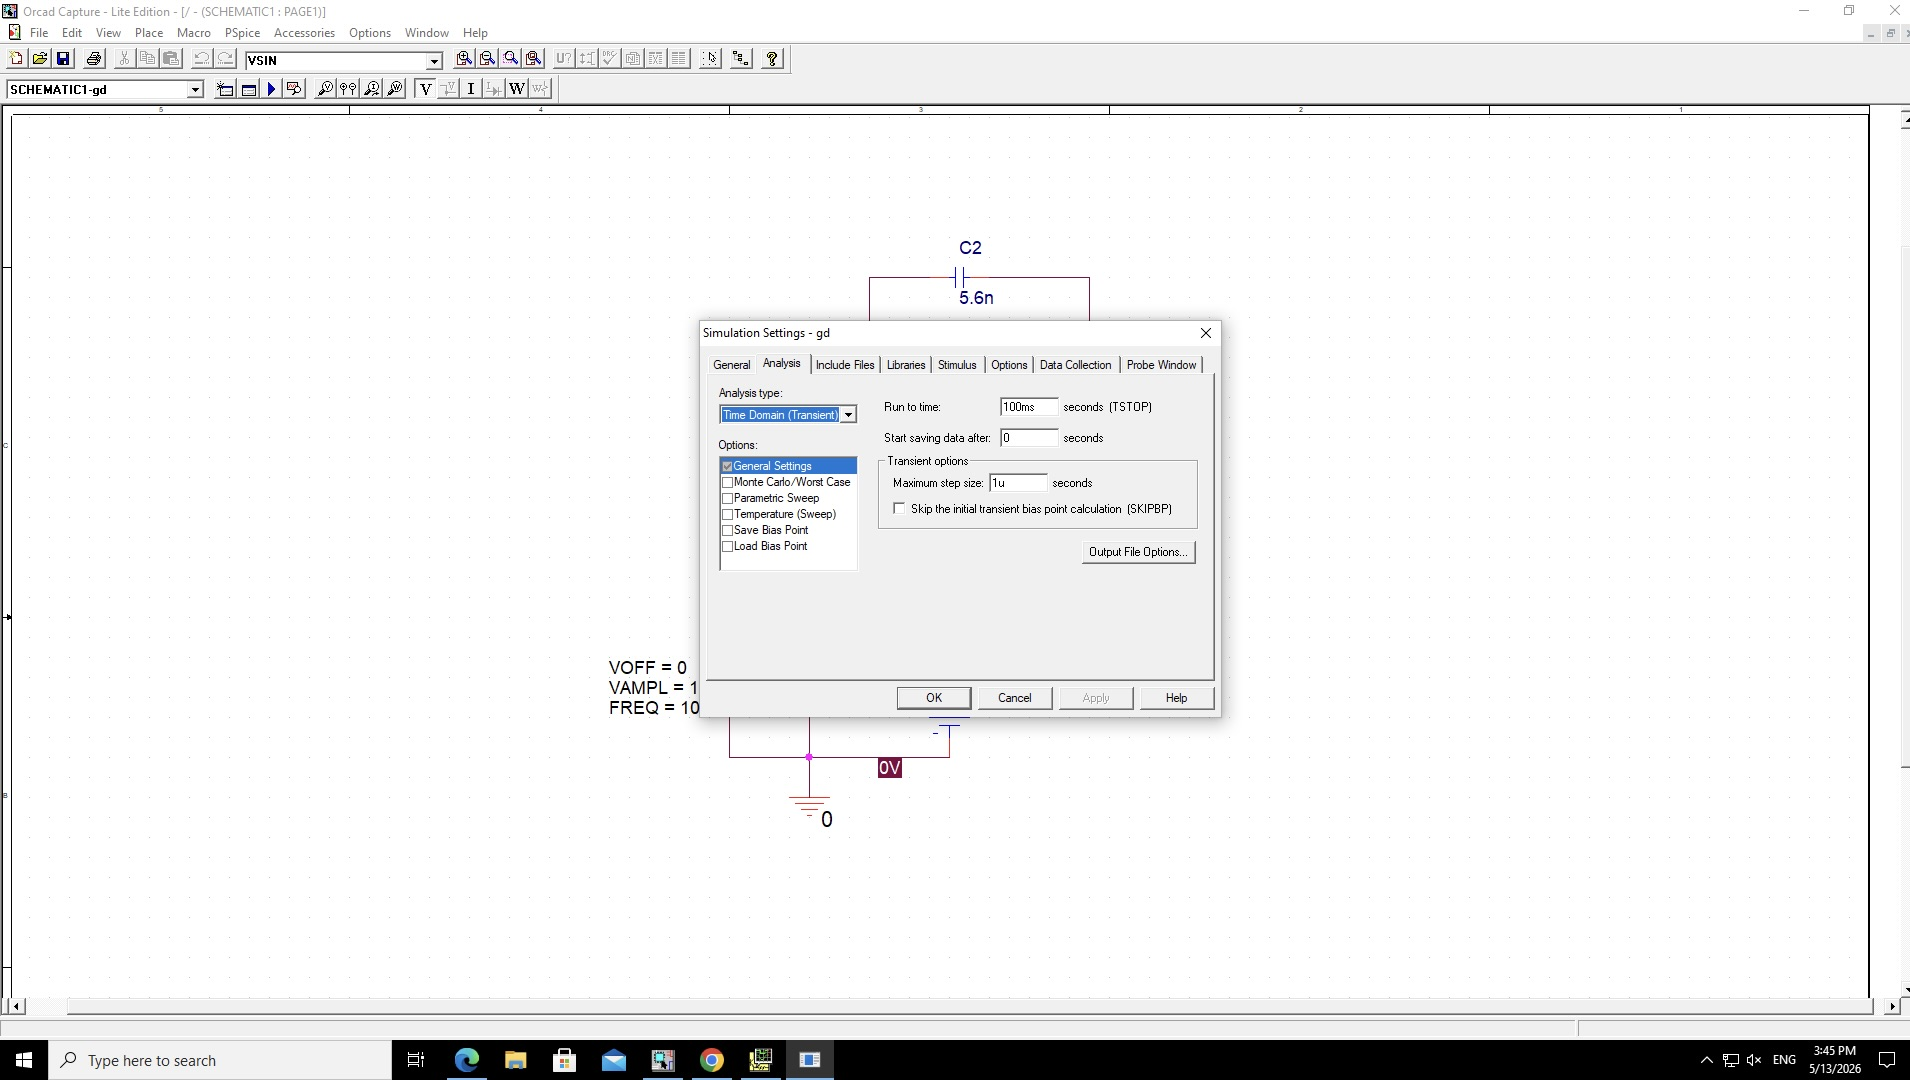
\includegraphics[width=\linewidth, keepaspectratio]{images/time_domain_prof.png}
            \caption{Time domain simulation profile settings as mentioned in the project description.}
            \label{fig:time}
        \end{minipage}
    }
\end{figure}

\clearpage
\section*{Simulation results:}
\subsection*{i. AC Sweep Simulation}
An AC sweep was performed to sketch the voltage gain magnitude versus frequency. As expected for a band-pass filter, the gain peaks at the center frequency and rolls off at higher and lower frequencies. The maximum gain is verified to be approximately 3.8 as calculated.

\begin{figure}[H]
    \centering
    \rotatebox{90}{
        \begin{minipage}{0.8\textheight} 
            \centering
            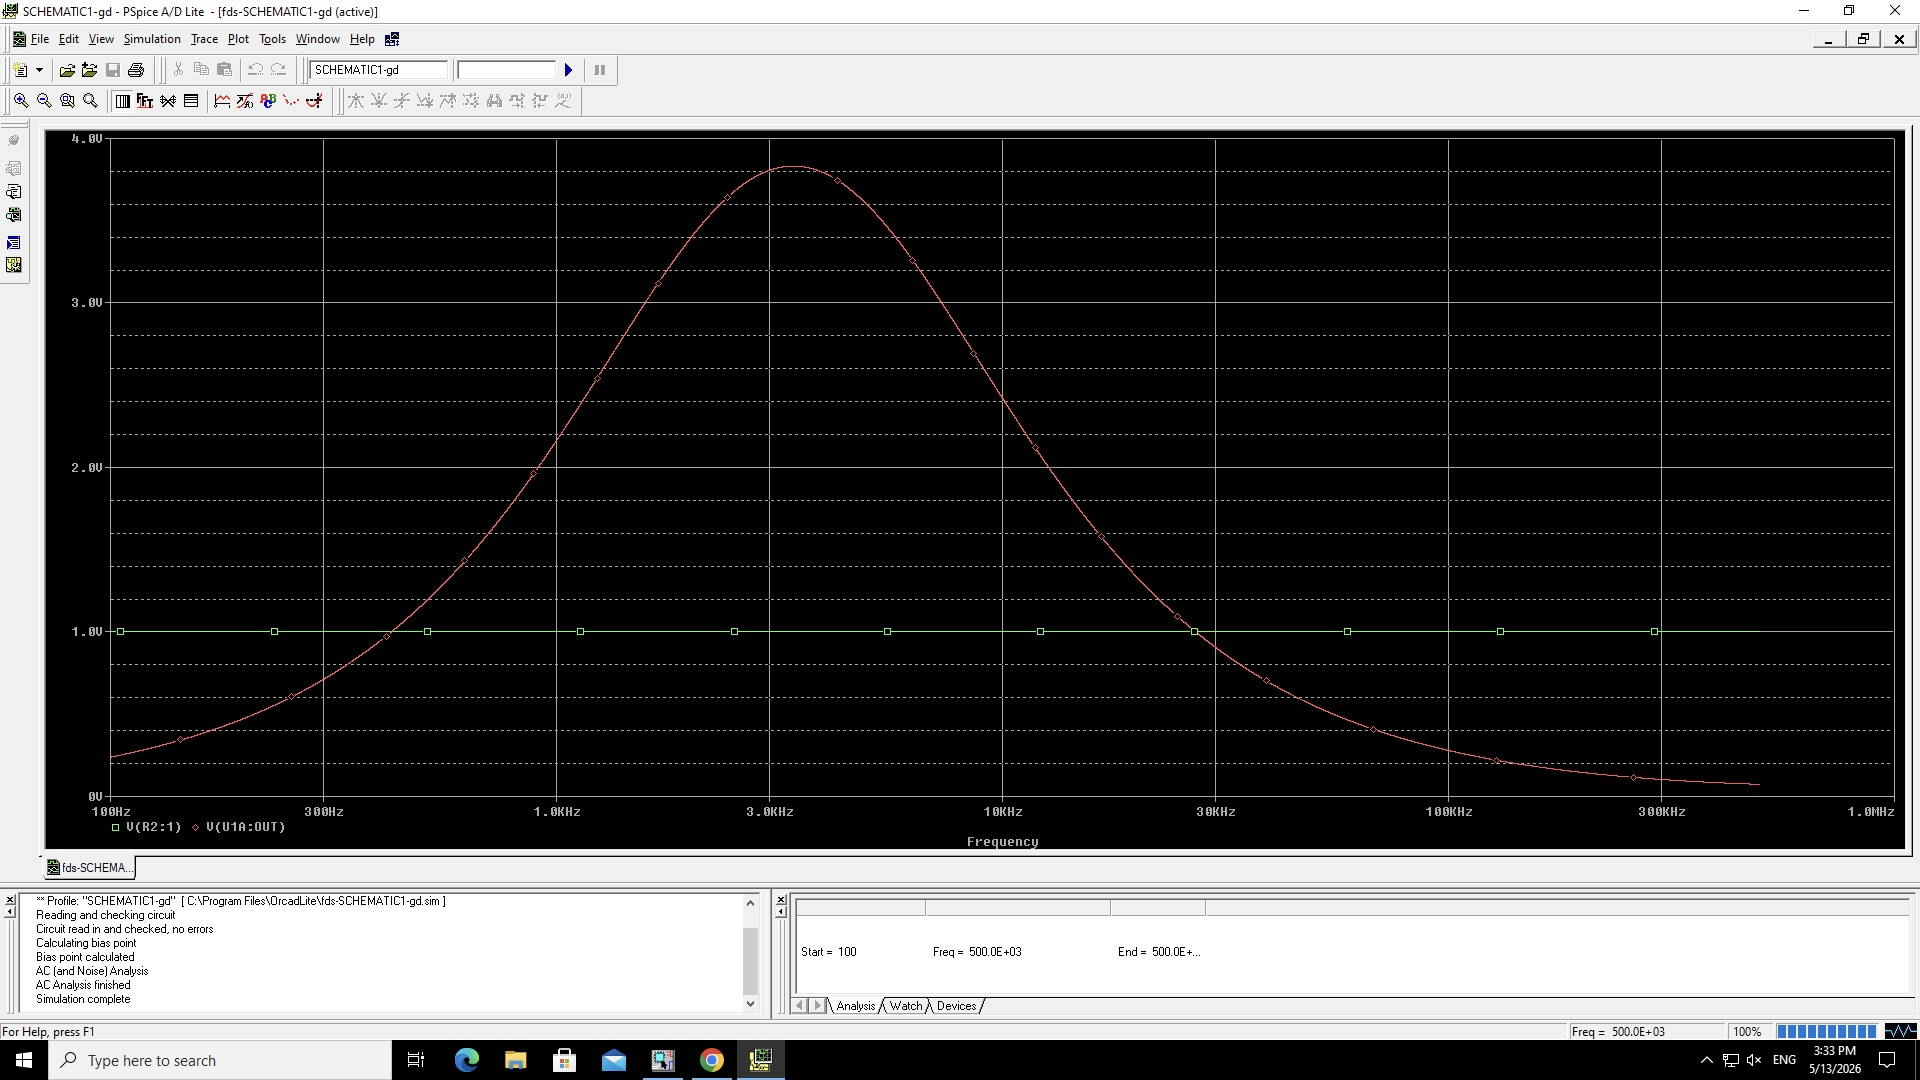
\includegraphics[width=\linewidth, keepaspectratio]{images/ac_sweep_graph.png}
            \caption{AC Sweep Simulation showing gain versus frequency.}
            \label{fig:ac_sweep}
        \end{minipage}
    }
\end{figure}

\clearpage
\subsection*{ii. Time Domain Simulation}
A time-domain analysis was conducted using a sinusoidal input voltage ($V_{sin}$) to observe the time-domain response. The output and input voltage amplitudes were compared at three different frequencies to demonstrate the band-pass attenuation characteristics.

% --- Time Domain: f < f0 ---
\begin{figure}[H]
    \centering
    \rotatebox{90}{
        \begin{minipage}{0.86\textheight} 
            \centering
            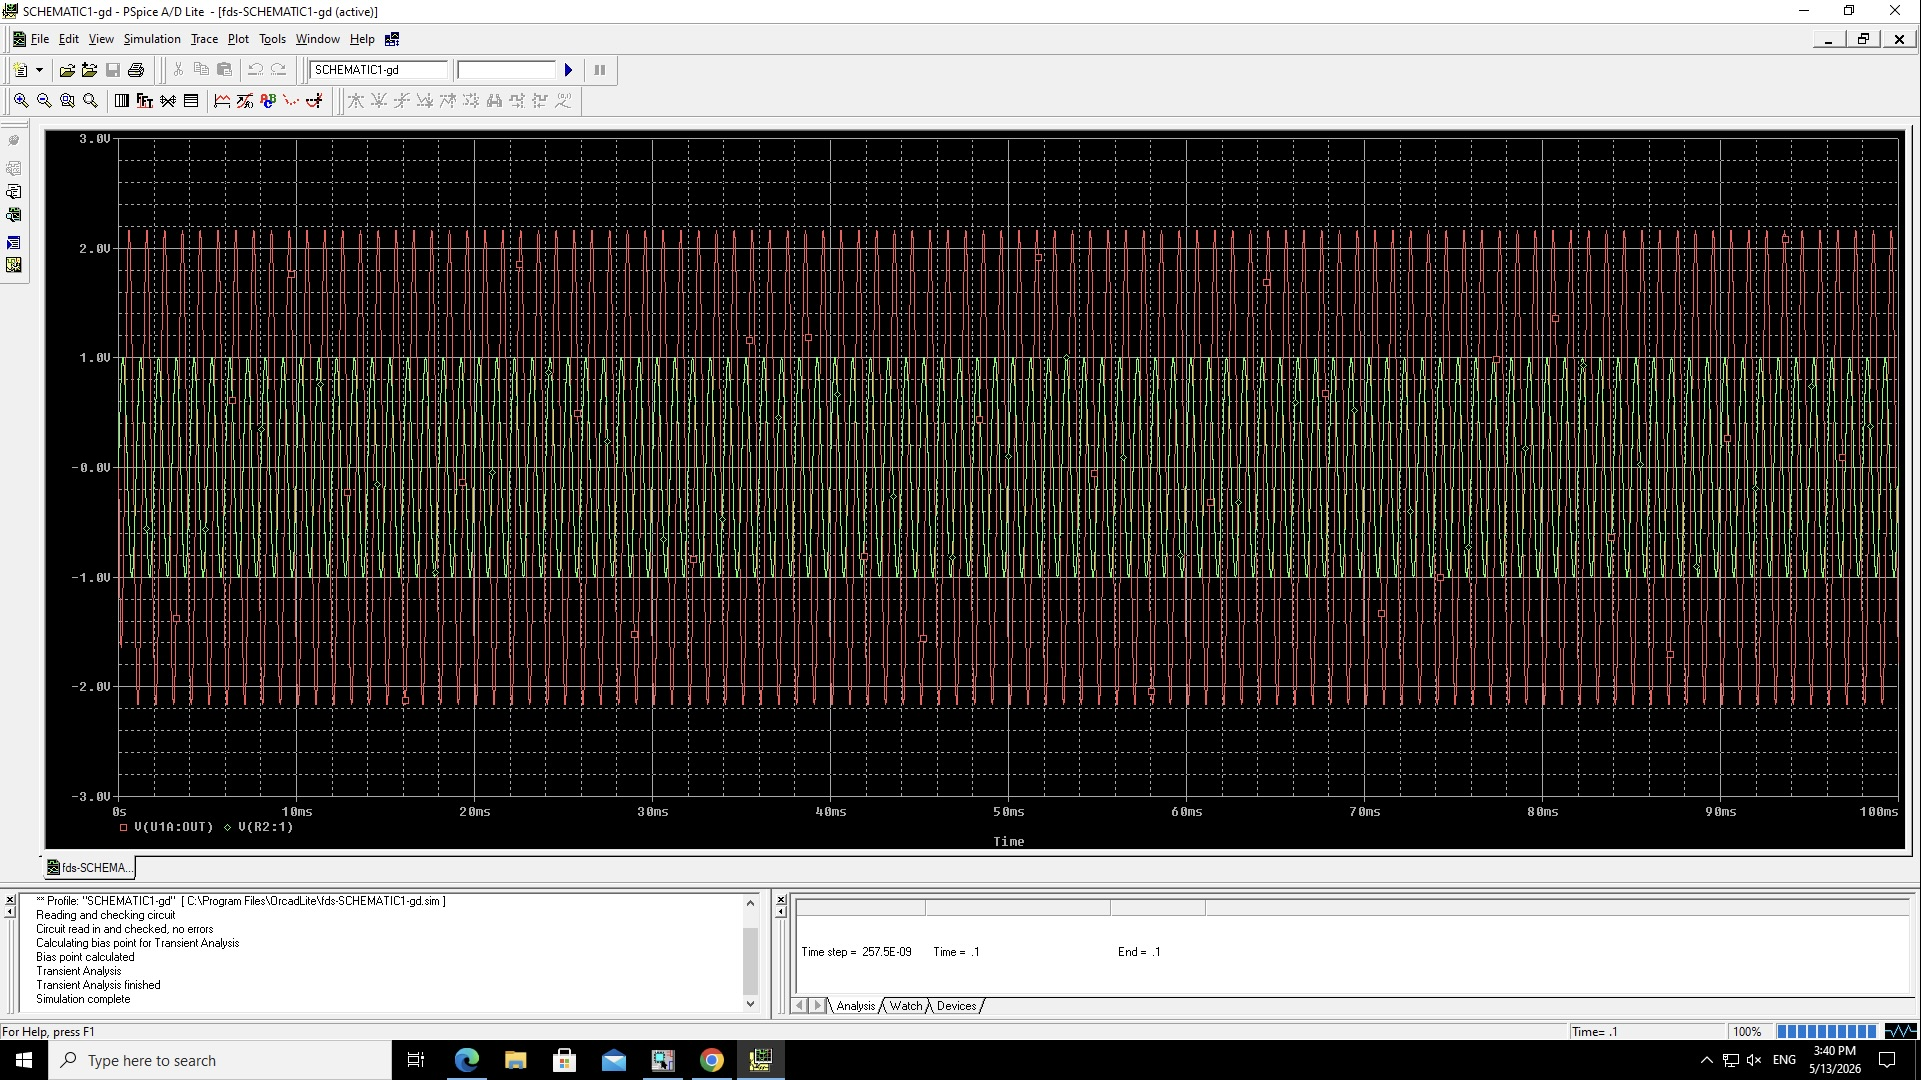
\includegraphics[width=\linewidth, keepaspectratio]{images/time_graph_1k.png}
            \caption{Time domain simulation at $f < f_0$ ($f = 1 \text{ kHz}$). The gain here is approximately 2.2 ($<3.8$) as expected from the AC sweep graph.}
            \label{fig:time_below}
        \end{minipage}
    }
\end{figure}

% --- Time Domain: f = f0 ---
\begin{figure}[H]
    \centering
    \rotatebox{90}{
        \begin{minipage}{1\textheight} 
            \centering
            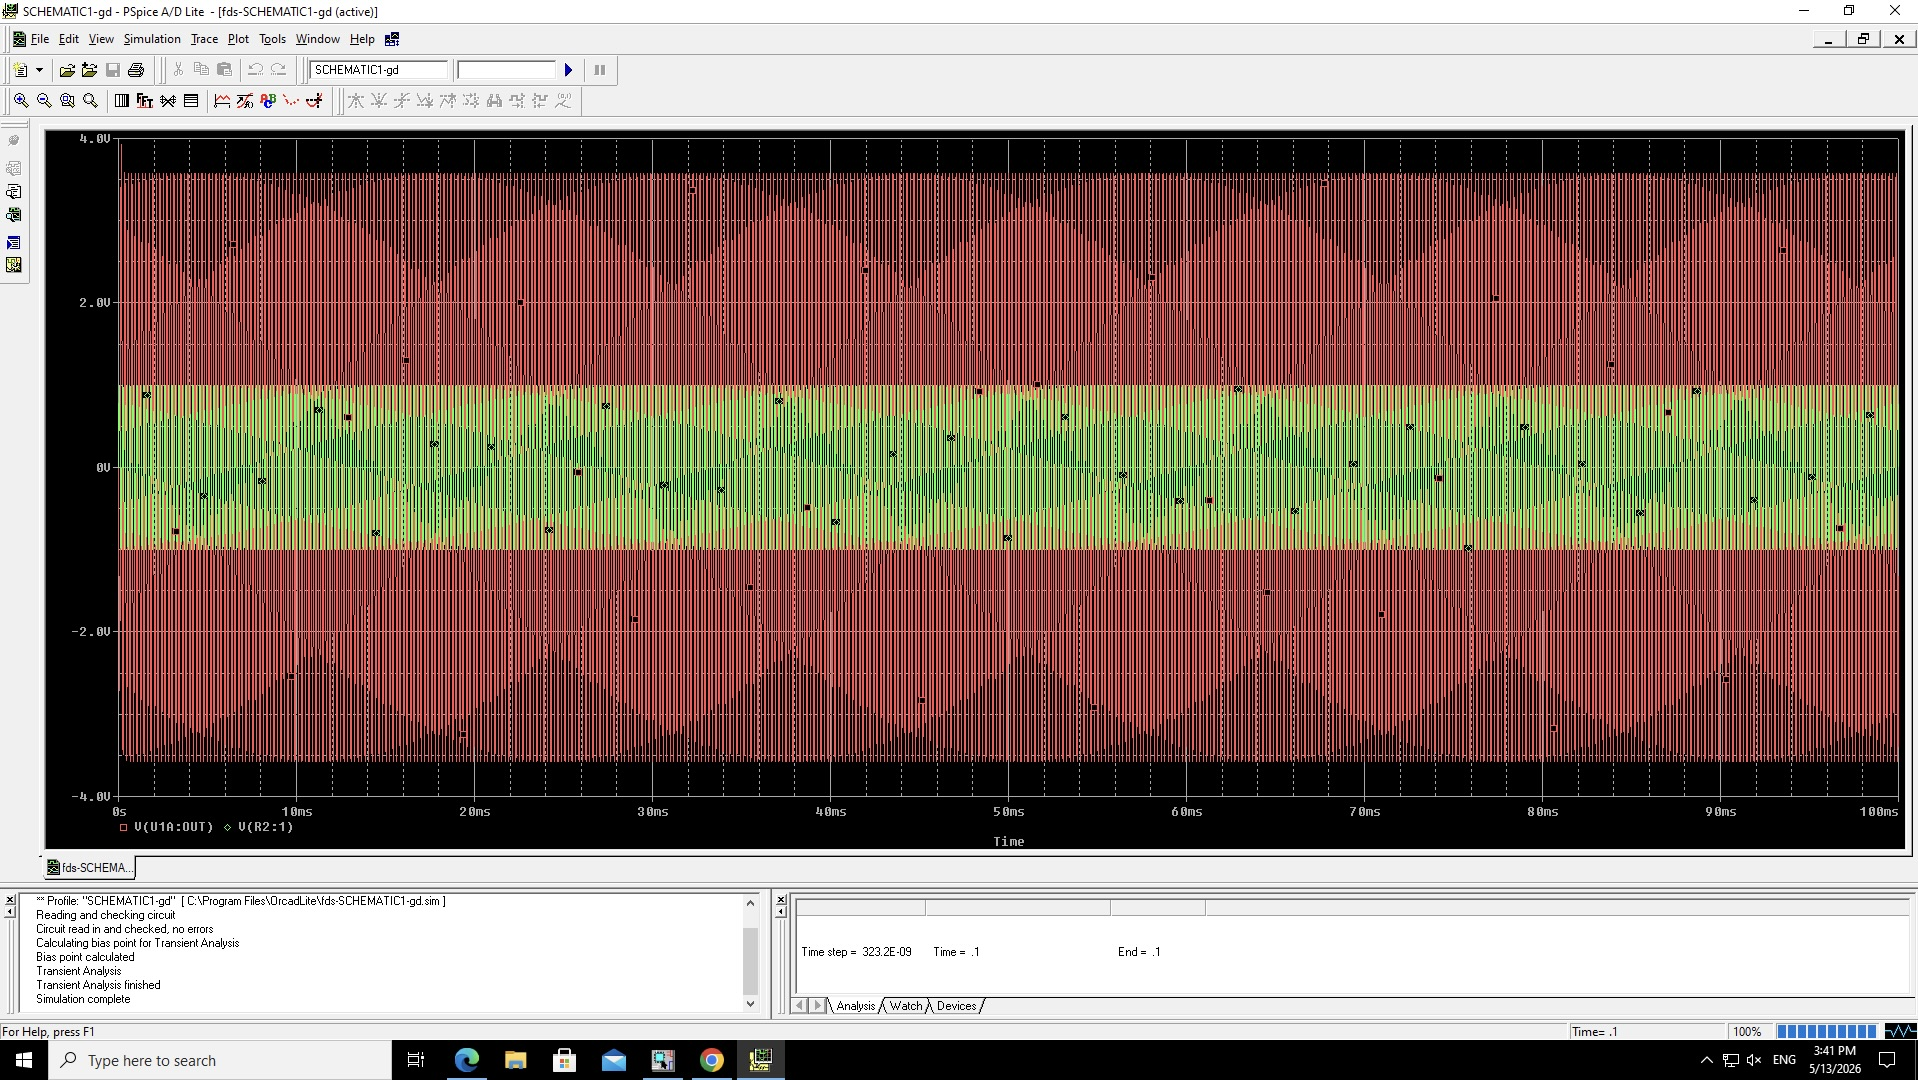
\includegraphics[width=\linewidth, keepaspectratio]{images/time_graph_f0.png}
            \caption{Time domain simulation at the resonant frequency $f = f_0 = 3.45 \text{ kHz}$. The gain here is approximately 3.8 as expected from the calculations.}
            \label{fig:time_center}
        \end{minipage}
    }
\end{figure}

% --- Time Domain: f > f0 ---
\begin{figure}[H]
    \centering
    \rotatebox{90}{
        \begin{minipage}{1\textheight} 
            \centering
            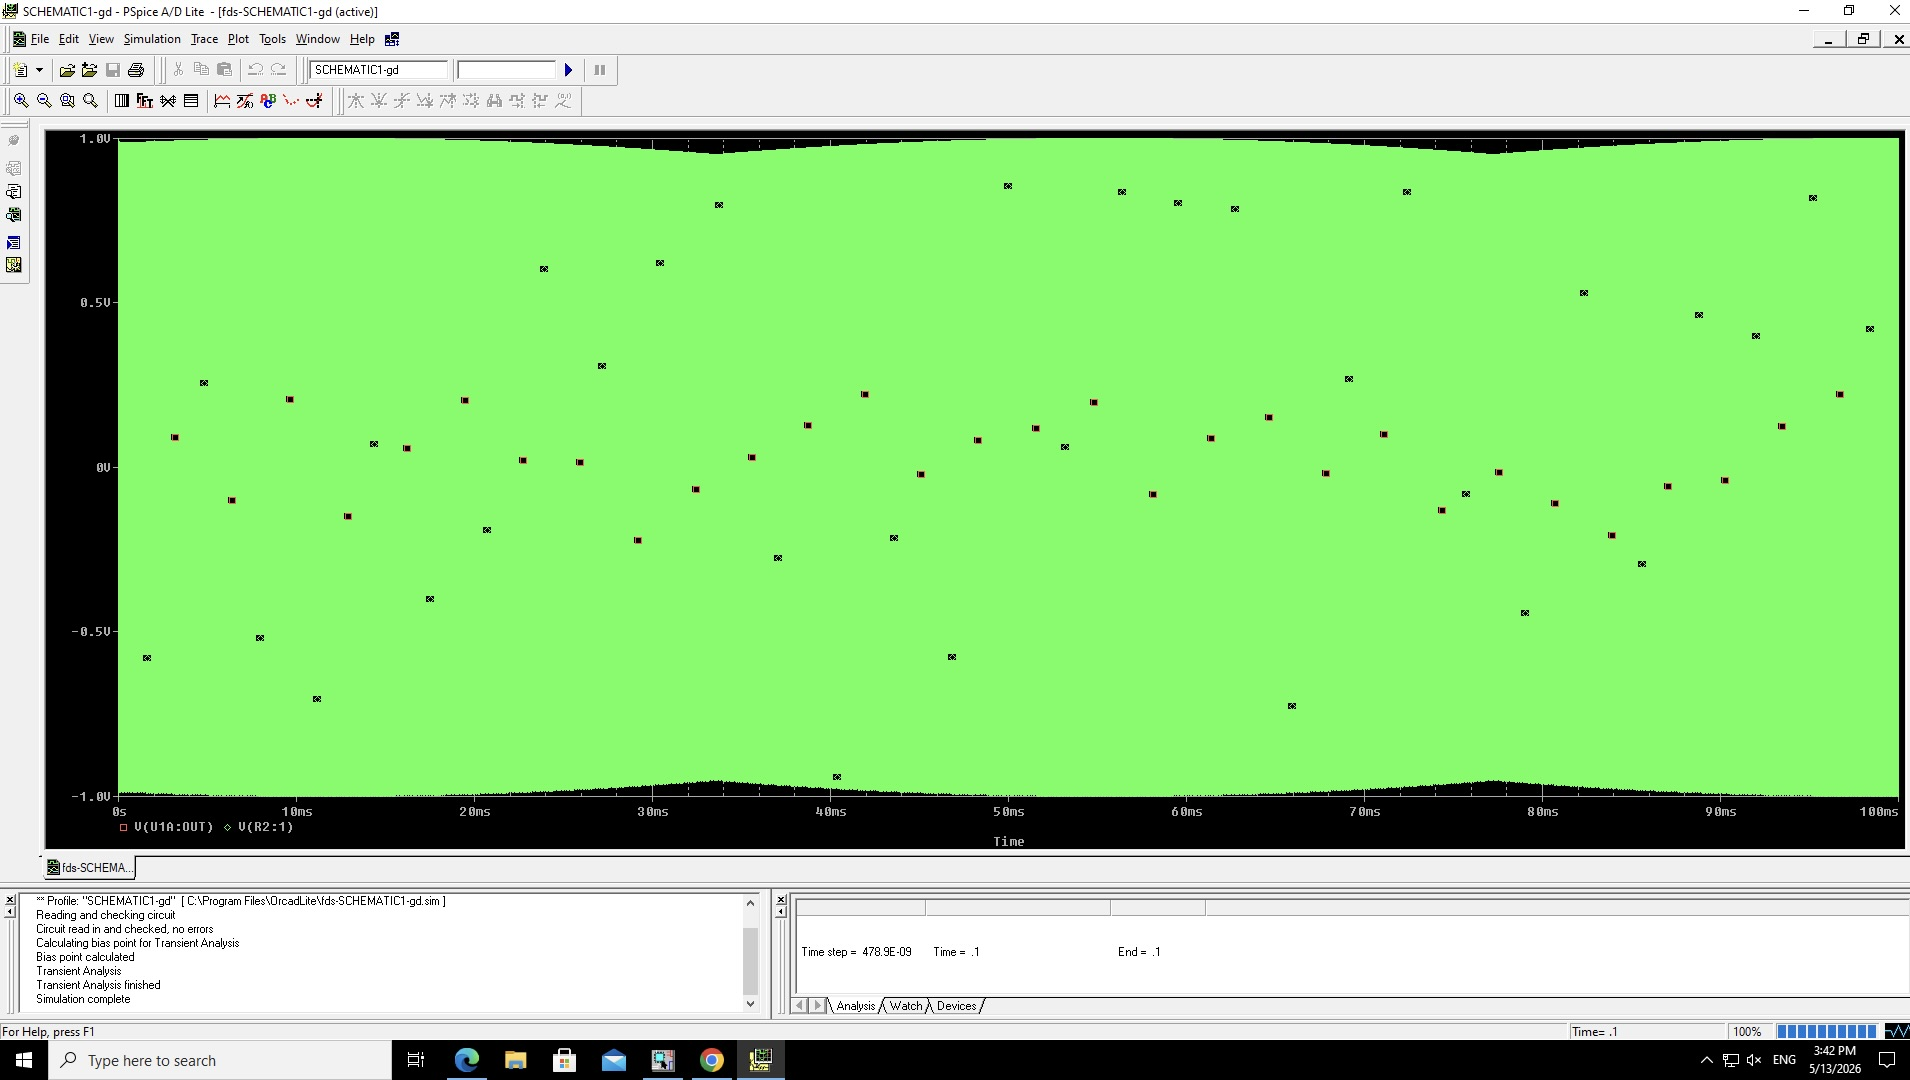
\includegraphics[width=\linewidth, keepaspectratio]{images/time_graph_100k.png}
            \caption{Time domain simulation at $f > f_0$ ($f = 100 \text{ kHz}$). We notice here that the red points ($V_{out}$) are below the green ones ($V_{in}$) meaning the gain is $<1$ as expected from the AC sweep graph.}
            \label{fig:time_above}
        \end{minipage}
    }
\end{figure}

\clearpage

\section*{Hardware implementation:}
The band-pass filter circuit was physically constructed on a standard breadboard for testing and validation. The details of the purchased components used for the hardware implementation are listed below, followed by photographs of the assembled circuit.

\subsection*{Purchased Components}

\begin{table}[h]
    \centering
    \begin{tabular}{|c|c|c|}
        \hline
        \textbf{Component} & \textbf{Nominal Value / Part Number} & \textbf{Quantity} \\
        \hline
        Resistor ($R_1$) & $1 \text{ k}\Omega$ & 1 \\
        \hline
        Resistor ($R_2$) & $5.6 \text{ k}\Omega$ & 1 \\
        \hline
        Capacitor ($C_1$) & $68 \text{ nF}$ & 1 \\
        \hline
        Capacitor ($C_2$) & $5.6 \text{ nF}$ & 1 \\
        \hline
        Operational Amplifier & LM741 & 1 \\
        \hline
    \end{tabular}
    \caption{List of components purchased for the hardware implementation.}
    \label{tab:components}
\end{table}

\vspace{.5cm} % Adds a little bit of spacing before the pictures

\subsection*{Hardware Pictures}
The physical circuit was wired according to the theoretical schematic.

% --- Hardware Image 1: Close up ---
\begin{figure}[H]
    \centering
    {
        \begin{minipage}{0.7\textheight} 
            \centering
            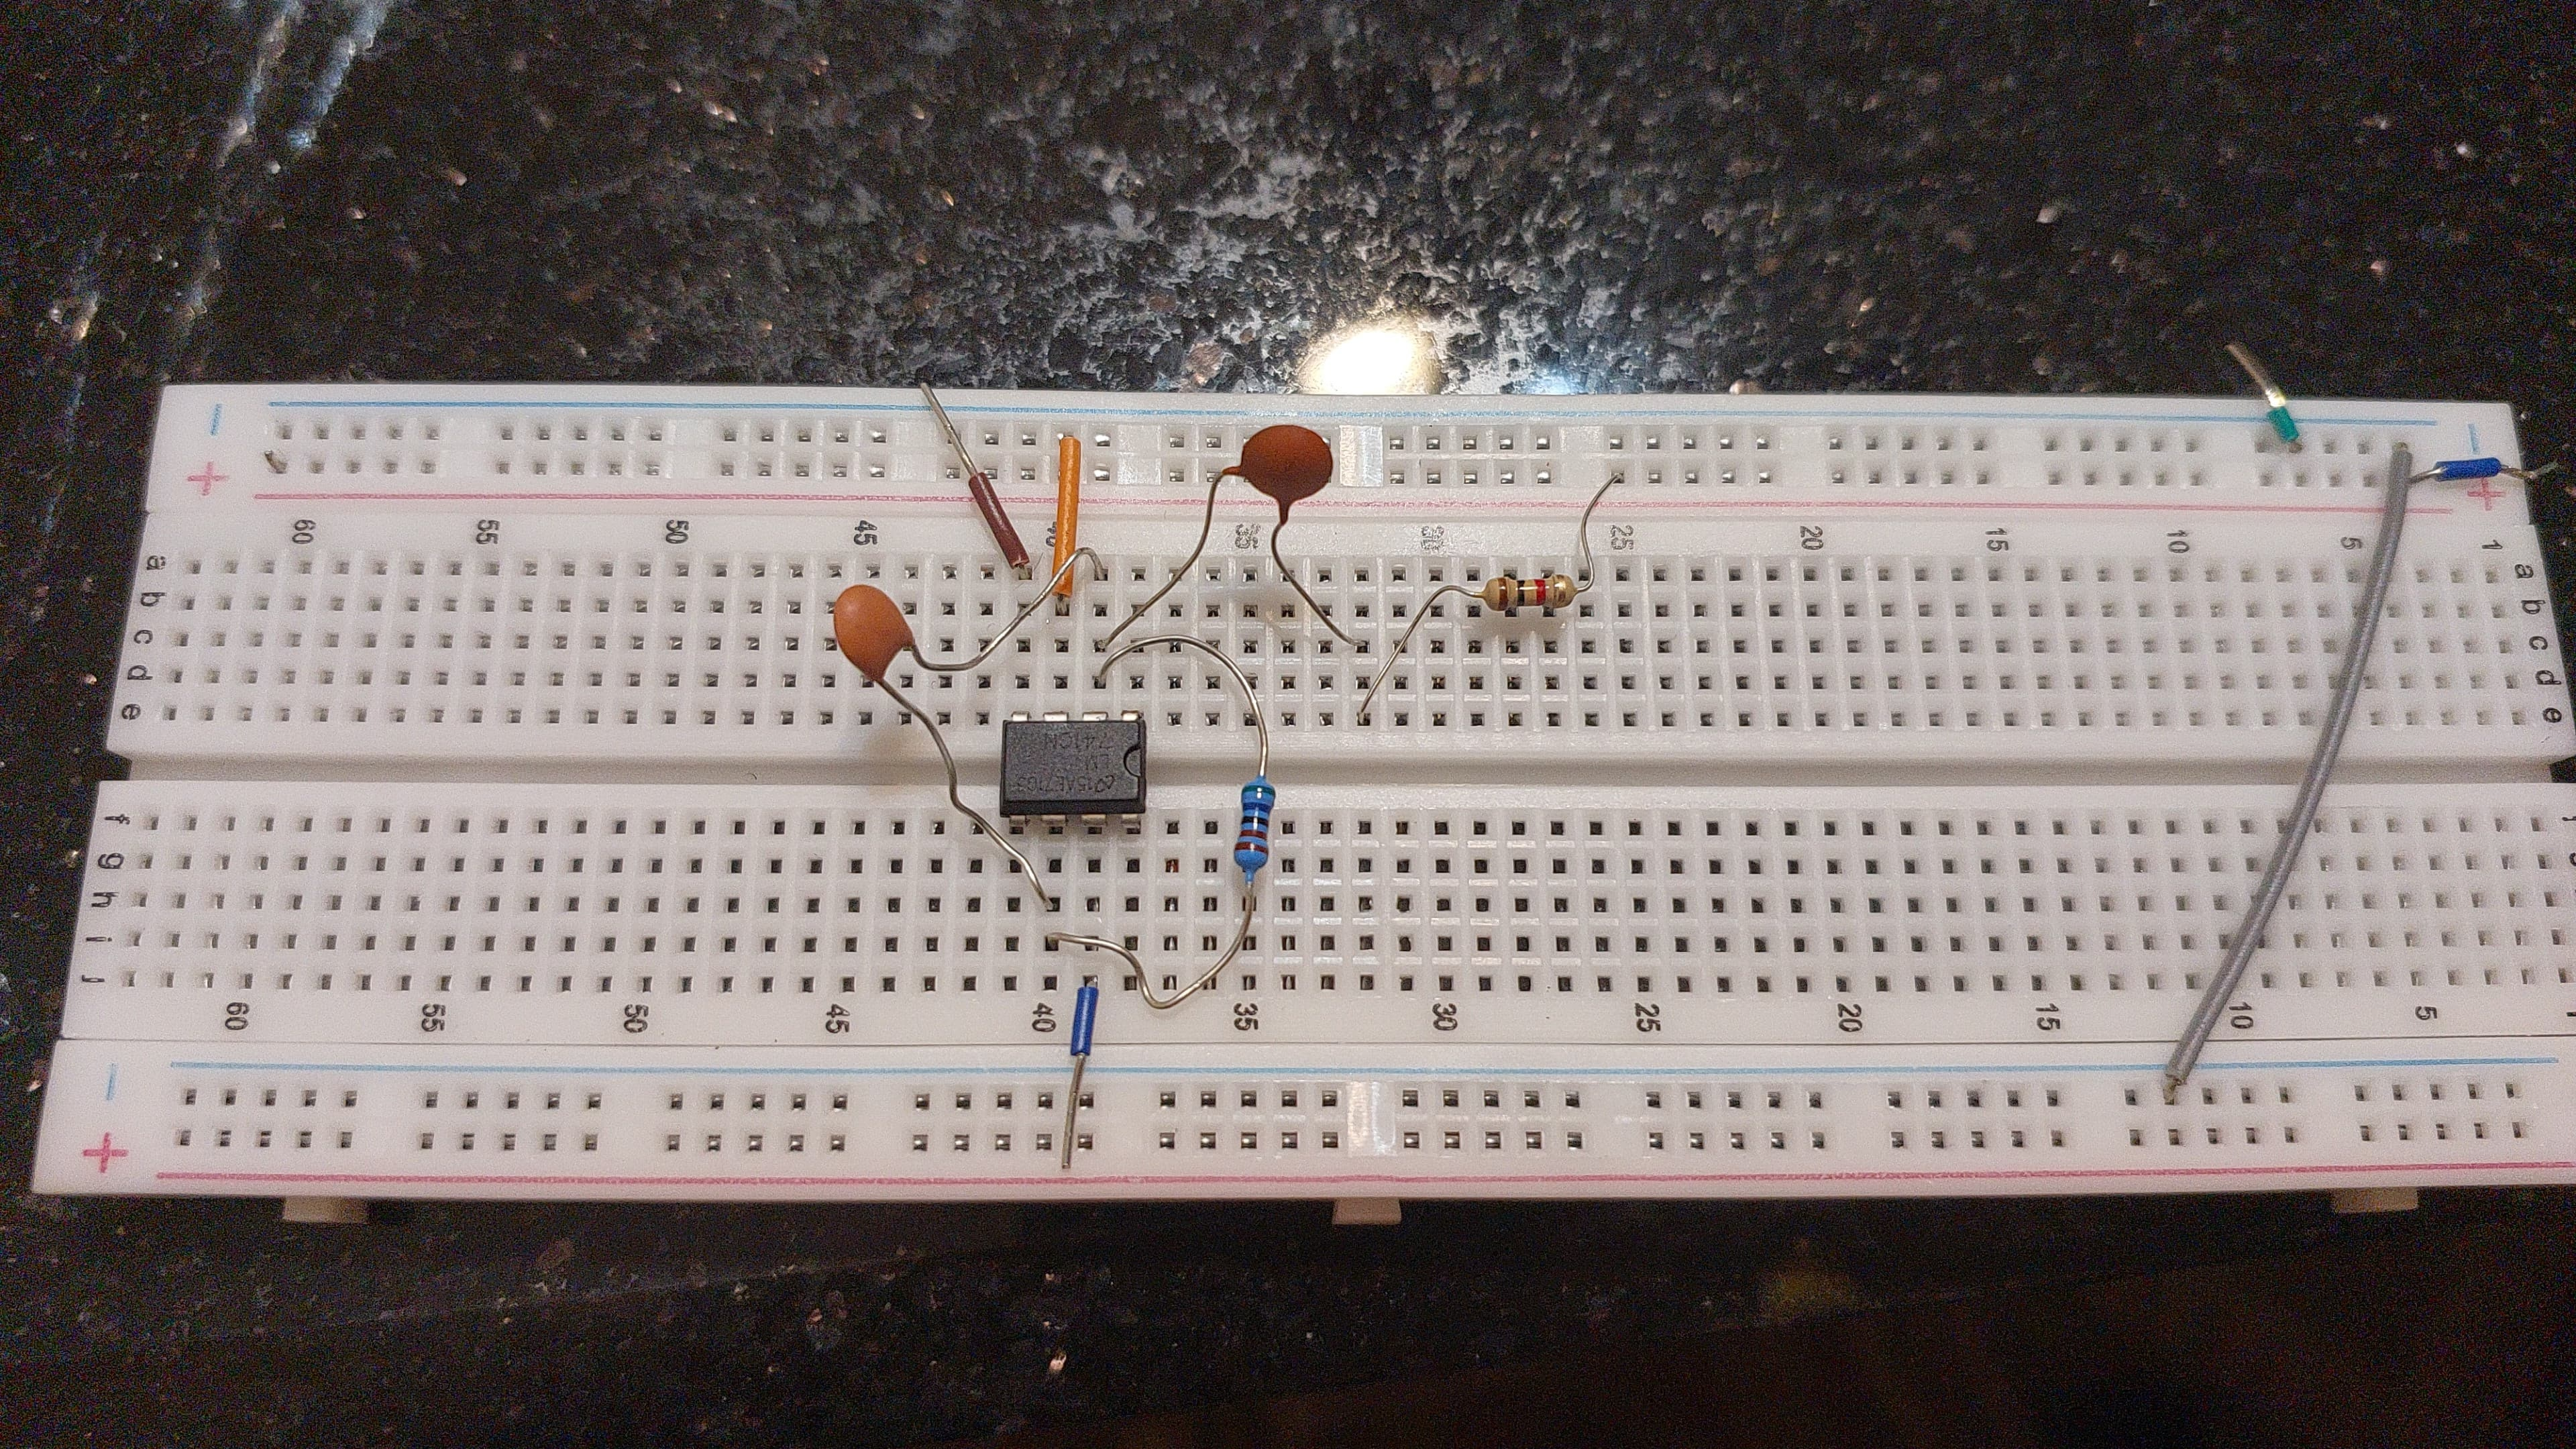
\includegraphics[width=\linewidth, keepaspectratio]{images/hard_circuit.png}
            \caption{Close-up view of the hardware implementation on the breadboard.}
            \label{fig:hardware_close}
        \end{minipage}
    }
\end{figure}

\clearpage

\section*{Hardware results:}
    To verify the physical operation of the filter, a function generator was used to supply a sinusoidal input signal ($V_{in}$), and a digital oscilloscope was used to simultaneously measure $V_{in}$ (Channel 1) and the output voltage $V_{out}$ (Channel 2).

The circuit was tested at three distinct frequencies relative to the calculated center frequency ($f_0 \approx 3.45 \text{ kHz}$) to observe the attenuation and amplification characteristics. Because this is an \textit{inverting} band-pass filter, a $180^\circ$ phase shift between the input and output signals is recognized.

\newpage
\subsection*{i. $f < f_0$ ($f = 1 \text{ kHz}$)}
At frequencies below the center frequency, the series input capacitor ($C_1$) exhibits high impedance, dominating the circuit and attenuating the input signal. The oscilloscope capture in Figure \ref{fig:hw_below} demonstrates this high-pass behavior, where the amplitude of $V_{out}$ is noticeably reduced compared to the expected maximum gain (gain is approximately 2 $<3.8$).

\begin{figure}[H]
    \centering
    \rotatebox{90}{
        \begin{minipage}{0.7\textheight} 
            \centering
            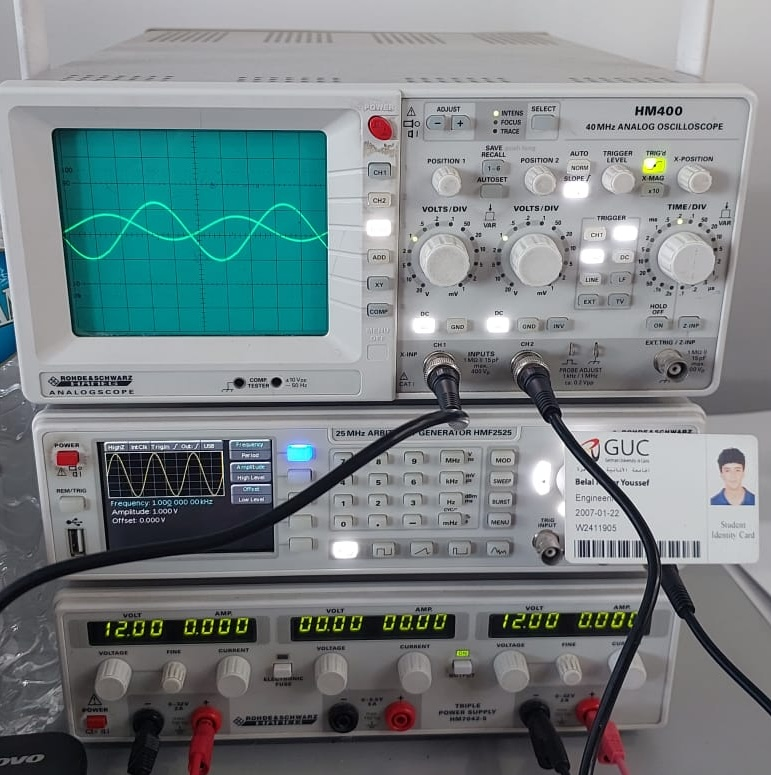
\includegraphics[width=\linewidth, keepaspectratio]{images/osc_1k.png}
            \caption{Oscilloscope capture at $f < f_0$. The output signal (CH2) shows attenuation.}
            \label{fig:hw_below}
        \end{minipage}
    }
\end{figure}
\newpage
\subsection*{ii. $f = f_0$ ($f = 3.45 \text{ kHz}$)}
At the center frequency, the reactive components balance, allowing the circuit to achieve its maximum voltage gain ($|H_{\max}|$). As seen in Figure \ref{fig:hw_center}, the output voltage reaches its peak amplitude. The measured ratio of $V_{out}$ to $V_{in}$ is approximately 3.2 which closely aligns with the theoretically calculated maximum gain of 3.83. The expected $180^\circ$ phase inversion is also clearly visible.

\begin{figure}[H]
    \centering
    \rotatebox{90}{
        \begin{minipage}{0.75\textheight} 
            \centering
            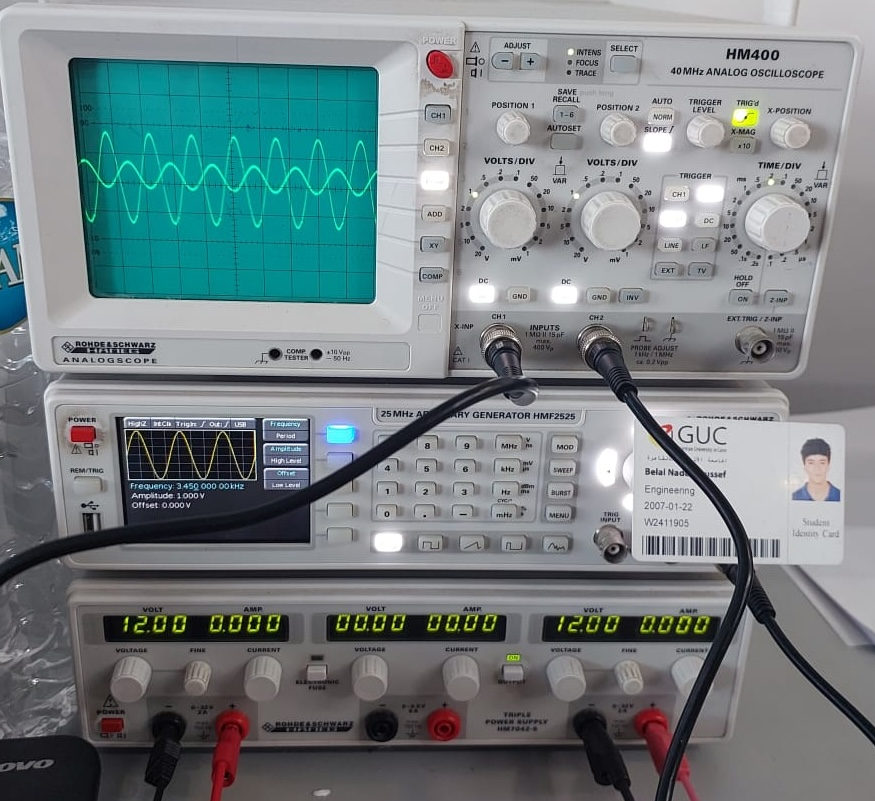
\includegraphics[width=\linewidth, keepaspectratio]{images/osc_f0.png}
            \caption{Oscilloscope capture at $f = f_0$. The circuit achieves maximum voltage gain.}
            \label{fig:hw_center}
        \end{minipage}
    }
\end{figure}

\subsection*{iii. $f > f_0$ ($f = 10 \text{ kHz}$)}
At frequencies above the center frequency, the parallel feedback capacitor ($C_2$) acts almost as a short circuit as the frequency increases, severely reducing the feedback impedance and pulling the output voltage toward the virtual ground. Figure \ref{fig:hw_above} illustrates this low-pass effect, showing significant attenuation of the output signal once again.

\begin{figure}[H]
    \centering
    \rotatebox{90}{
        \begin{minipage}{0.75\textheight} 
            \centering
            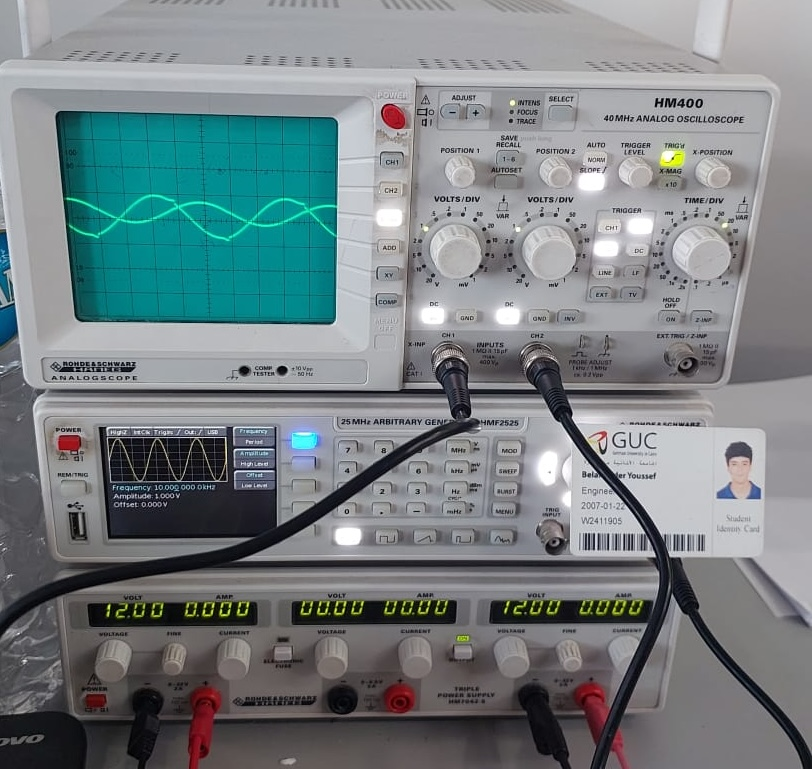
\includegraphics[width=\linewidth, keepaspectratio]{images/osc_10k.png}
            \caption{Oscilloscope capture at $f > f_0$. The output signal (CH2) is heavily attenuated.}
            \label{fig:hw_above}
        \end{minipage}
    }
\end{figure}

\newpage
\subsection*{Discussion of Results}
The hardware implementation successfully validates the theoretical design and PSpice simulations. By observing the amplitude of $V_{out}$ across the frequency spectrum, it is evident that the circuit allows a specific band of frequencies to pass with amplification (peaking at $f_0 = 3.45 \text{ kHz}$) while attenuating frequencies outside this range. This behavior, coupled with the observed phase inversion, conclusively demonstrates that the constructed circuit functions as an Inverting Active Band-Pass Filter.

\end{document}